\documentclass{article}

\usepackage{fancyhdr}
\usepackage{extramarks}
\usepackage{amsmath}
\usepackage{amsthm}
\usepackage{amsfonts}
\usepackage{tikz}
\usepackage[plain]{algorithm}
\usepackage{algpseudocode}
\usepackage{graphicx}
\graphicspath{{./images/}}

\usetikzlibrary{automata,positioning}

%
% Basic Document Settings
%

\topmargin=-0.45in
\evensidemargin=0in
\oddsidemargin=0in
\textwidth=6.5in
\textheight=9.0in
\headsep=0.25in

\linespread{1.1}

\pagestyle{fancy}
\lhead{\hmwkAuthorName}
\chead{\hmwkClass\ (\hmwkClassInstructor\ \hmwkClassTime): \hmwkTitle}
\rhead{\firstxmark}
\lfoot{\lastxmark}
\cfoot{\thepage}

\renewcommand\headrulewidth{0.4pt}
\renewcommand\footrulewidth{0.4pt}

\setlength\parindent{0pt}

%
% Create Problem Sections
%

\newcommand{\enterProblemHeader}[1]{
    \nobreak\extramarks{}{Problem \arabic{#1} continued on next page\ldots}\nobreak{}
    \nobreak\extramarks{Problem \arabic{#1} (continued)}{Problem \arabic{#1} continued on next page\ldots}\nobreak{}
}

\newcommand{\exitProblemHeader}[1]{
    \nobreak\extramarks{Problem \arabic{#1} (continued)}{Problem \arabic{#1} continued on next page\ldots}\nobreak{}
    \stepcounter{#1}
    \nobreak\extramarks{Problem \arabic{#1}}{}\nobreak{}
}

\setcounter{secnumdepth}{0}
\newcounter{partCounter}
\newcounter{homeworkProblemCounter}
\setcounter{homeworkProblemCounter}{1}
\nobreak\extramarks{Problem \arabic{homeworkProblemCounter}}{}\nobreak{}

%
% Homework Problem Environment
%
% This environment takes an optional argument. When given, it will adjust the
% problem counter. This is useful for when the problems given for your
% assignment aren't sequential. See the last 3 problems of this template for an
% example.
%
\newenvironment{homeworkProblem}[1][-1]{
    \ifnum#1>0
        \setcounter{homeworkProblemCounter}{#1}
    \fi
    \section{Problem \arabic{homeworkProblemCounter}}
    \setcounter{partCounter}{1}
    \enterProblemHeader{homeworkProblemCounter}
}{
    \exitProblemHeader{homeworkProblemCounter}
}

%
% Homework Details
%   - Title
%   - Due date
%   - Class
%   - Section/Time
%   - Instructor
%   - Author
%

\newcommand{\hmwkTitle}{Assignment\ \#3}
\newcommand{\hmwkDueDate}{September 22, 2022}
\newcommand{\hmwkClass}{Formal}
\newcommand{\hmwkClassTime}{4:10 PM}
\newcommand{\hmwkClassInstructor}{Professor Matthew Patitz}
\newcommand{\hmwkAuthorName}{\textbf{Piam Chittisane}}

%
% Title Page
%

\title{
    \vspace{2in}
    \textmd{\textbf{\hmwkClass:\ \hmwkTitle}}\\
    \normalsize\vspace{0.1in}\small{Due\ on\ \hmwkDueDate\ at 11:59pm}\\
    \vspace{0.1in}\large{\textit{\hmwkClassInstructor\ \hmwkClassTime}}
    \vspace{3in}
}

\author{\hmwkAuthorName}
\date{}

\renewcommand{\part}[1]{\textbf{\large Part \Alph{partCounter}}\stepcounter{partCounter}\\}

%
% Various Helper Commands
%

% Useful for algorithms
\newcommand{\alg}[1]{\textsc{\bfseries \footnotesize #1}}

% For derivatives
\newcommand{\deriv}[1]{\frac{\mathrm{d}}{\mathrm{d}x} (#1)}

% For partial derivatives
\newcommand{\pderiv}[2]{\frac{\partial}{\partial #1} (#2)}

% Integral dx
\newcommand{\dx}{\mathrm{d}x}

% Alias for the Solution section header
\newcommand{\solution}{\textbf{\large Solution}}

% Probability commands: Expectation, Variance, Covariance, Bias
\newcommand{\E}{\mathrm{E}}
\newcommand{\Var}{\mathrm{Var}}
\newcommand{\Cov}{\mathrm{Cov}}
\newcommand{\Bias}{\mathrm{Bias}}

\begin{document}

\maketitle

\pagebreak

\begin{homeworkProblem}
    Prove Theorem 1 (i.e. if L is a regular language, then $\overline{L}=\Sigma^*/L$ is also regular).
    \\
    \solution
    \\
    If L is a regular language, that must mean there is a DFA $M=(Q,\Sigma,\delta,q_0,F)$ that recognizes the language.
    Since $\overline{L}$ accepts any expression that isn't accepted by $L$, all that needs to be done is complement the accepting states.
    DFA $\overline{M}=(Q,\Sigma,\delta,q_0,Q/F)$ should exist such that $L(\overline{M})=\overline{L}$.
\end{homeworkProblem}

\begin{homeworkProblem}
    Give regular expressions generating the following languages. In all parts, the alphabet is \{0, 1\}.
    \\
    \part{}
    $\{w \mid \text{every odd position of } w \text{ is a } 1\}$
    \\
    \solution
    \\
    $R=(1\Sigma)^*$
    \\
    \part{}
    $\{w \mid w \text{ contains at least two 0s and at most one 1}\}$
    \\
    \solution
    \\
    $R=000^*+((01+10)0+000^*1)0^*$
    

\end{homeworkProblem}

\begin{homeworkProblem}
    Use the procedure described in Lemma 1.55 to covert the following regular expressions to nondeterministic finite automata.
    \\
    \part{}
    $(0\cup1)^*000(0\cup1)^*$
    \\
    \solution
    \\
    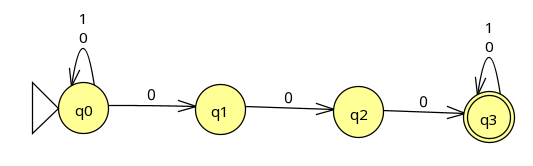
\includegraphics[scale=0.50]{3a.png}
    \\
    \part{}
    $(((00)^*(11)) \cup 01)^*$
    \\
    \solution
    \\
    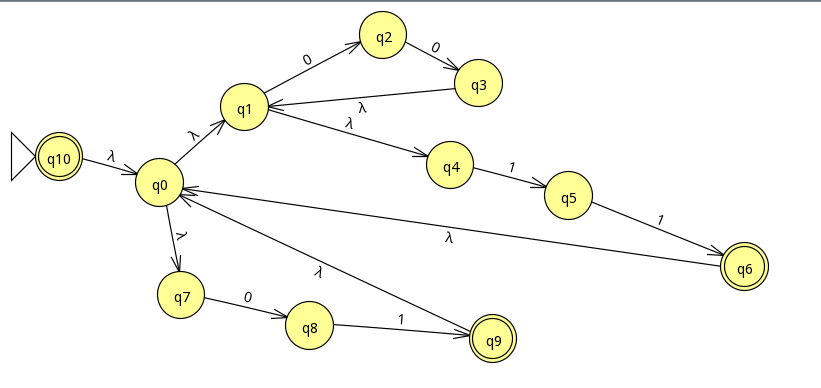
\includegraphics[scale=0.42]{3b.png}
\end{homeworkProblem}

\pagebreak

\begin{homeworkProblem}
    Use the procedure described in Lemma 1.60 to covert the following finite automata to regular expressions.
    \part{}
    \\
    \solution
    \\
    $(a^*ba^*b)^*a^*ba^*$
    \\
    \part{}
    \\
    \solution
    \\
    $((a\cup b)a^*b(ba^*b)^*a)^*(\epsilon\cup(a\cup b)a^*b(ba^*b)^*)$
\end{homeworkProblem}

\begin{homeworkProblem}
    Let $\Sigma=\{0,1,+,=\}$ and
    $ADD = \{x=y+z \mid x,y,z \text{ are binary integers, and } x \text{ is the sum of } y \text { and } z \}$
    \\ Prove that ADD is not regular.
    \\
    \solution
    \begin{proof}
        Let string $s$ be $1^p=1^p+0^p$. Since $1^p$ is as long as the pumping length $p$, the substring $y$ must consist of only 1s. For any arbitrary $y$, if $y$ is pumped down (if $y=0$), the equality of $x=y+z$ does not hold since there will be less 1s in $x$ than $y$.
    \end{proof}
\end{homeworkProblem}

\begin{homeworkProblem}
    Prove that the following language is not regular. You may use the pumping lemma and the closure of the class of regular languages under union, intersection, and complement.
    $\{w\mid w \in \{0, 1\}^* \text{ is not a palindrome}\}$
    \\
    \solution
    \begin{proof}
        Assume the language $L$ is regular.\\
        The language $\overline{L}$ = $\{w \mid w \in \{0,1\}^* \text{ is a palindrome}\}$ must be regular due to closure under complement. \\
        Consider the string $0^p10^p$ that is accepted by $\overline{L}$. \\
        Since $0^p$ is as long as the pumping length $p$, the substring $y$ must only consist of 0s. \\
        If substring $y$ is pumped up or pumped down, the number of 0s before 1 will not equal the number of 0s after, resulting in a whole string that isn't a palindrome. \\
        Therefore, $\overline{L}$ is not a regular language.
        If $\overline{L}$ is not a regular language, $L$ is not a regular language through closure, resulting in a proof by contradiction.


    \end{proof}
\end{homeworkProblem}

\end{document}
